\documentclass[12pt]{article}
\usepackage{makeidx}
\usepackage{hyperref}
\usepackage{graphicx}
\usepackage{lmodern}
\usepackage[T1]{fontenc}
\usepackage{geometry}
\geometry{margin=1in}
\newcommand{\candidate}[2]{#1} % TODO: fix this to better have hierarchical indexing? 
\makeindex

\title{Recreational Computing: \\The Joy of Machines for Their Own Sake}
\author{}
\date{\today}

\begin{document}
\maketitle

\begin{minipage}{0.15\textwidth}
    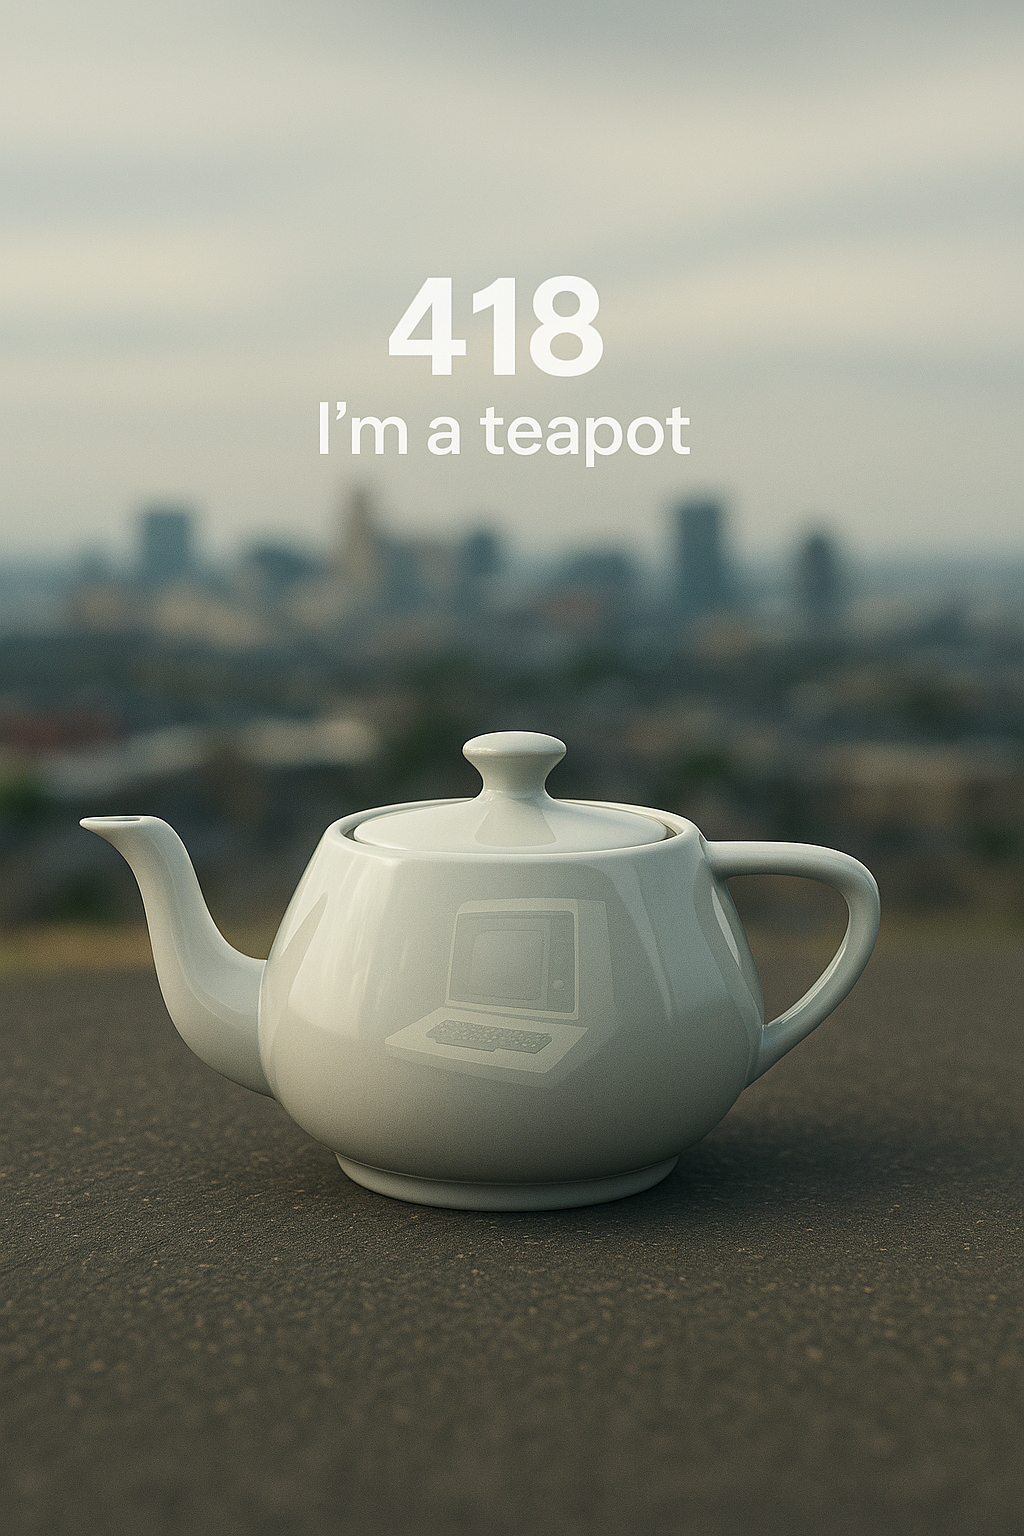
\includegraphics[width=\textwidth]{./teapot.png} % Include your QR code image file
\end{minipage}

\subsection*{Introduction}
There is an entire universe of computing that exists not for productivity, not for profit, but purely for the love of the machine itself---a kind of \textit{recreational computing}\index{recreational computing}, where the act of tinkering, exploring, or even deliberately wasting cycles is the point.

\subsection*{Demoscene: Code as Art}
In the 1980s, groups of programmers and hackers began competing to create the most visually stunning or technically impressive audiovisual displays---known as demos\index{demoscene}. These works, often just kilobytes in size, pushed hardware beyond its intended limits, bending sound chips into makeshift synthesisers and exploiting raster tricks to render 3D graphics on machines never designed for it. 

Today, demoscene culture thrives, with competitions like \textit{Revision}\index{Revision (demoscene competition)} drawing coders who write assembly by hand, not because it’s practical, but because it’s \textit{beautiful}.

\subsection*{Esolangs: Programming for the Absurd}
Some programmers design languages not to be useful, but to be \textit{interesting}. Esoteric programming languages (esolangs)\index{esolangs} like \textit{Brainfuck}, \textit{Whitespace}, or \textit{Malbolge}\index{Brainfuck}\index{Whitespace}\index{Malbolge} exist purely as intellectual exercises. Writing a \texttt{Hello, World!} in these languages is a puzzle, a joke, or sometimes a form of computational poetry.

\subsection*{Useless Machines and Infinite Loops}
From \textbf{Quine}\index{Quine} programs (which print their own source code) to \textit{fork bombs}\index{fork bomb} (a single line of code that spawns processes until a system crashes), there’s a subculture of computing dedicated to recursive, paradoxical, or deliberately ``pointless'' constructs. Some enthusiasts build physical \textit{useless machines}\index{useless machine}---boxes with a single switch that, when flipped, trigger a mechanical arm to turn itself off again. The entire exercise is a meditation on the absurdity of automation.

\subsection*{Retrocomputing as a Hobby}
For some, the joy lies in resurrecting old hardware---not for nostalgia, but for the challenge. Getting a \textit{1970s mainframe}\index{mainframe!1970s} to run modern networking protocols, or fitting an entire Linux distribution onto a \textit{floppy disk}\index{floppy disk}, is a game of constraints. Others deliberately slow down modern machines to match the pace of early home computers, finding satisfaction in the limitations themselves.

\subsection*{Generative Art and Algorithmic Play}
Tools like \textit{Processing}, \textit{PICO-8}, or \textit{Shadertoy}\index{Processing}\index{PICO-8}\index{Shadertoy} turn programming into a canvas. The goal isn’t efficiency---it’s \emph{emergence}. A few lines of code can produce infinite fractal landscapes, chaotic pendulum simulations, or glitchy pixel animations. Some programmers spend hours tweaking procedural algorithms just to see what unexpected beauty (or chaos) unfolds.

\subsection*{The Joy of Over-Engineering}
Why write a simple script when you could deploy a \textit{Kubernetes cluster}\index{Kubernetes} to serve a single static HTML page? Why use a calculator when you could pipe numbers through a \textit{custom LISP interpreter}\index{LISP interpreter}? Recreational computing embraces the unnecessarily complex, the ornate, the \emph{delightfully excessive}---not because it’s better, but because the journey is the point.

\subsection*{Why Does It Matter?}
Recreational computing is a reminder that technology isn’t just a tool---it’s a \textit{toy}. Before computers were for work, they were for play: the early hackers at MIT\index{MIT} wrote games before they wrote operating systems. In an age where software is increasingly optimised for profit, recreational computing keeps alive the spirit of curiosity, of bending systems just to see what happens.

It’s the digital equivalent of building sandcastles---elaborate, temporary, and utterly pointless. And that’s exactly what makes it worthwhile.

\newpage
\printindex

\end{document}